\begin{figure}
    \begin{center}
    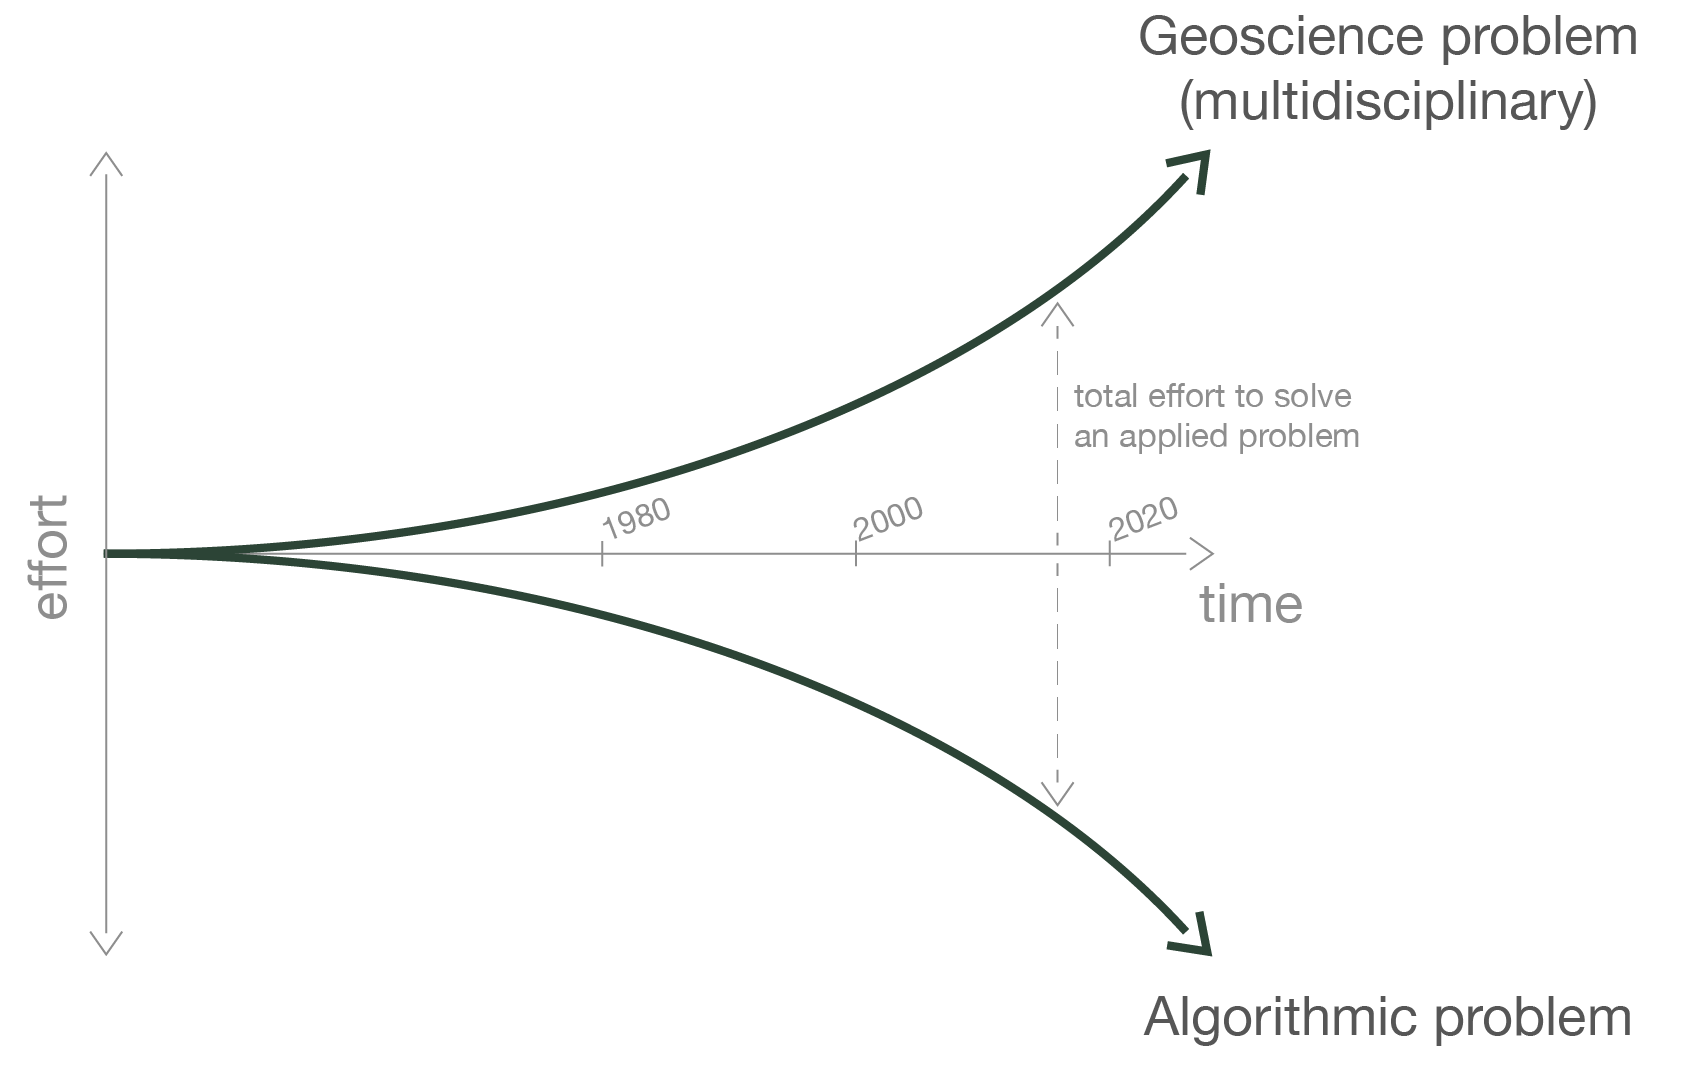
\includegraphics[width=0.8\columnwidth]{figures/diverging-curves-08.png}
    \end{center}
\caption{
    The plight of a researcher in geoscience. The horizontal axis reflects time, and
    the vertical distance away from this axis reflects the effort a researcher must
    invest in order to solve a problem. The lower curve represents the effort required
    to solve an algorithmic problem and the upper curve represents the effort required
    to solve an integrated geoscience problem that involves multiple disciplines.
    The distance between these two curves at any point in time represents the total
    effort required to solve an applied geoscience problem at the state-of-the-art,
    as these problems require both algorithmic components and multidisciplinary
    interpretations.
}
\label{fig:diverging-curves}
\end{figure}
